\mychapter{0}{Introduction}
%\addcontentsline{toc}{section}{Introduction}
\markboth{Introduction}{Introduction}
%\label{chap:introduction}
%\minitoc

This report describes a study of events where a photon and an hadronic jet are produced in proton-proton 
collisions recorded by the Compact Muon Solenoid (CMS) at the Large Hadron Collider (LHC).\\

The LHC at CERN collides protons at a record energy of 13TeV since 2016, and CMS is one of the multi-purpose 
detector installed at one of the LHC interaction points to study the products of such collisions.\\

High-energy quarks and gluons are produced in such collisions, and are observed in the detectors as hadronic jets. 
Hadronic jets are a flagship observable for QCD studies and are heavily used in most analysis at the LHC (from 
precision measurements of Standard Model parameters to searches for physics beyond the Standard Model). 
Due to their complex nature, they are one of the less precisely reconstructed objects at the LHC, and a 
dedicated community of experimentalists and theorists is dedicated to their studies.\\
Events where a photon and a jet are produced are very useful for studying the jet properties thanks to the high
precision 
with which CMS measures photons. Fig (\ref{gamma_jet}) shows one of the Feynman diagrams describing, at LO, the production of such
events. 
Unfortunately, it is hard to select samples with a very high fraction of photon+jet events, 
due to the presence of a background coming from multijet events (produced at at much higher rate) where one jet is 
wrongly identified as a photon. Until now, the purity of photon+jet samples has been determined based on simulations.\\

This report documents a study for a data-driven technique for extracting the gamma+jet purity, based on several photon 
identification observables, combined in a multivariate technique.\\

%At the Compact Muon Solenoid are produced at high-energy, proton-proton collision. At these energy scale quarks and
%gluons interact to form a collimated jet of hadrons, called hadronics jets
%This phenomenon allow us to probe the QCD and the proton structure, but is very complexe to analyze.\\
%One way to measure jets energy is to study \textgamma+jet events, on fig (\ref{gamma_jet}) the photon is prompt and balance the jet energy.

\begin{figure}[h!]
  \centering
  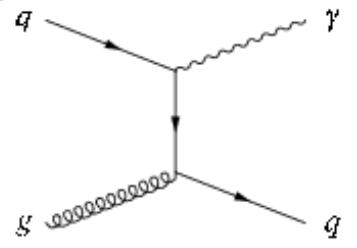
\includegraphics[width=0.4\textwidth]{gamma_jet}\\[1cm]
  \caption{Feynman diagram of a quark-gluon interaction, giving in output a high-energy quark and a prompt photon.}
  \label{gamma_jet}
\end{figure}

This report describes the analysis of \textgamma+jet events, in the first section will be described the CMS detector and
the hadronic jets. Then will be introduced the data that have been used for the analysis part.
For the analysis part will be implemented a multivariate analysis for photon identification this will be used for
measuring the \textgamma+jet purity in the data.

%%% Local Variables: 
%%% mode: latex
%%% TeX-master: "isae-report-template"
%%% End: 
